\documentclass[12pt,a4paper]{report}
\usepackage[utf8]{inputenc}
\usepackage[english]{babel}
\usepackage{graphicx}
\usepackage{geometry}
\geometry{a4paper, margin=1in}
\usepackage{setspace}
\onehalfspacing
\usepackage{times} % Times New Roman
\usepackage{fancyhdr}
\usepackage{multirow}
\usepackage{array}
\usepackage{colortbl}
\usepackage{xcolor}
\usepackage{listings}
\usepackage{hyperref}
\usepackage{indentfirst} % Indent the first paragraph of sections

% Custom page style for the final template metadata page
\fancypagestyle{lastpage}{
  \fancyhf{}
  \fancyfoot[C]{\thepage}
  \renewcommand{\headrulewidth}{0pt}
  \renewcommand{\footrulewidth}{0pt}
}

% Define custom colors
\definecolor{ganttblue}{HTML}{1F4E79}
\definecolor{codegray}{rgb}{0.95,0.95,0.95}
\definecolor{codeblue}{rgb}{0.1,0.1,0.6}
\definecolor{codegreen}{rgb}{0,0.5,0}

% Code listing styles
\lstdefinelanguage{JavaScript}{
  keywords={break, case, catch, continue, debugger, default, delete, do, else, false, finally, for, function, if, in, instanceof, new, null, return, switch, this, throw, true, try, typeof, var, void, while, with, const, let, class, export, import, from, extends},
  morekeywords={require, module, exports},
  ndkeywords={class, export, boolean, throw, implements, import, this},
  ndkeywordstyle=\color{darkgray}\bfseries,
  identifierstyle=\color{black},
  sensitive=false,
  comment=[l]{//},
  morecomment=[s]{/*}{*/},
  commentstyle=\color{codegreen}\itshape,
  stringstyle=\color{red}\ttfamily,
  morestring=[b]',
  morestring=[b]"
}

\lstset{
  backgroundcolor=\color{codegray},
  basicstyle=\ttfamily\small,
  breaklines=true,
  captionpos=b,
  commentstyle=\color{codegreen}\itshape,
  keywordstyle=\color{codeblue}\boldfamily,
  stringstyle=\color{red},
  showstringspaces=false,
  frame=single,
  numbers=none,
  tabsize=2
}

% Standard links styling
\hypersetup{
    colorlinks=true,
    linkcolor=blue,      % Blue links for Table of Contents, figures, and cross-references
    filecolor=blue,      
    urlcolor=blue,
    citecolor=blue
}

\begin{document}

% ==========================================
% PAGE 1: COVER PAGE
% ==========================================
\begin{titlepage}
    \centering
    \vspace*{1cm}
    
    {\fontsize{18}{22}\selectfont \textbf{Design and Development of a Modern MERN Stack E-Commerce Platform} \par}
    
    \vspace{2cm}
    {\fontsize{12}{14}\selectfont An Internship Report\\Submitted in partial fulfillment of the requirements for the Degree of\\Bachelor of Science in Computer Science and Engineering \par}
    
    \vspace{1.5cm}
    {\fontsize{12}{14}\selectfont Submitted by\par}
    \vspace{0.3cm}
    {\fontsize{12}{14}\selectfont \textbf{Raisa Tabassum Kabir \quad 2022100000032} \par}
    
    \vspace{1.5cm}
    {\fontsize{12}{14}\selectfont Supervised by\par}
    \vspace{0.3cm}
    {\fontsize{12}{14}\selectfont \textbf{Radiathun Tasnia}\\Lecturer\\Department of Computer Science and Engineering\\Southeast University \par}
    
    \vspace{1.5cm}
    
\includegraphics[width=0.3\textwidth]{images/seu_logo.png}
    
    \vfill
    {\fontsize{12}{14}\selectfont \textbf{Department of Computer Science and Engineering}\\ \textbf{Southeast University}\\Dhaka, Bangladesh\\ \textbf{July 06, 2026} \par}
\end{titlepage}

\pagenumbering{roman}
\pagestyle{plain}

% ==========================================
% PAGE 2: LETTER OF TRANSMITTAL
% ==========================================
\newpage
\addcontentsline{toc}{chapter}{\textit{LETTER OF TRANSMITTAL}}
\begin{center}
    {\fontsize{14}{16}\selectfont \textbf{Letter of Transmittal}}
\end{center}
\vspace{1cm}

\noindent July 06, 2026 \\\\
The Chairman,\\
Department of Computer Science and Engineering\\
Southeast University\\
Tejgaon, Dhaka, Bangladesh\\\\
Through: Supervisor, Radiathun Tasnia\\\\
Subject: Submission of Internship Report.\\\\
Dear Sir,\\
With due respect, I am pleased to submit my internship report entitled ``Design and Development of a Modern MERN Stack E-Commerce Platform'' in partial fulfillment of the requirements for completing the internship program.

During my internship at Fionetix Solutions, I worked as a Software Developer (Intern) on developing an end-to-end pipeline for a modern e-commerce web application. The framework combines a React frontend, Node.js and Express backend, MongoDB database, secure Stripe payment processing, and Cloudinary media management.

This report provides an overview of the tasks I performed, the methodologies I followed, the tools and technologies I used and the key learnings gained throughout the internship. I have prepared this report carefully according to the given instructions and requirements.

Thank you for your support and consideration.

\vspace{1.5cm}
\noindent
\begin{minipage}[t]{0.45\textwidth}
Sincerely Yours,\\
\vspace{1.5cm}\\
\rule{5cm}{0.4pt}\\
\textbf{Raisa Tabassum Kabir}\\
2022100000032
\end{minipage}
\hfill
\begin{minipage}[t]{0.45\textwidth}
Supervisor:\\
\vspace{1.5cm}\\
\rule{5cm}{0.4pt}\\
\textbf{Radiathun Tasnia}\\
Lecturer \& Supervisor\\
Department of Computer Science\\
and Engineering\\
Southeast University
\end{minipage}

% ==========================================
% PAGE 3: CANDIDATE'S DECLARATION
% ==========================================
\newpage
\addcontentsline{toc}{chapter}{\textit{CANDIDATES' DECLARATION}}
\begin{center}
    {\fontsize{14}{16}\selectfont \textbf{CANDIDATE'S DECLARATION}}
\end{center}
\vspace{1.5cm}

\noindent I, hereby, declare that the thesis presented in this report is the outcome of the investigation performed by us under the supervision of Radiathun Tasnia, Lecturer, Department of Computer Science and Engineering, Southeast University. The work was done through CSE489: Internship course, in accordance with the course curriculum of the Department for the Bachelor of Science in Computer Science and Engineering program.

It is also declared that neither this research nor any part thereof has been submitted anywhere else for the award of any degree, diploma or other qualifications.

\vspace{3cm}
\noindent
\rule{5cm}{0.4pt}\\
\textbf{Raisa Tabassum Kabir}\\
2022100000032

% ==========================================
% PAGE 4: CERTIFICATION
% ==========================================
\newpage
\addcontentsline{toc}{chapter}{\textit{CERTIFICATION}}
\begin{center}
    {\fontsize{14}{16}\selectfont \textbf{CERTIFICATION}}
\end{center}
\vspace{1.5cm}

\noindent This report titled, ``Design and Development of a Modern MERN Stack E-Commerce Platform'', submitted by the people mentioned below has been accepted as satisfactory in partial fulfillment of the requirements for the degree B.Sc. in Computer Science and Engineering in July 2026.

\vspace{1cm}
\noindent \textbf{Member:}\\
\vspace{0.2cm}
\noindent \textbf{Raisa Tabassum Kabir \quad 2022100000032}

\vspace{2.5cm}
\noindent
\begin{minipage}[t]{0.45\textwidth}
\rule{5cm}{0.4pt}\\
Radiathun Tasnia\\
Lecturer \& Supervisor\\
Department of Computer Science\\
and Engineering\\
Southeast University
\end{minipage}
\hfill
\begin{minipage}[t]{0.45\textwidth}
\rule{5cm}{0.4pt}\\
Fatimatuj Johora\\
Chief Operating Officer (COO)\\
Fionetix Solutions
\end{minipage}

\vspace{2.5cm}
\noindent
\begin{minipage}[t]{0.45\textwidth}
\rule{5cm}{0.4pt}\\
Shahriar Manzoor\\
Associate Professor \& Chairman\\
Department of Computer Science\\
and Engineering\\
Southeast University
\end{minipage}

% ==========================================
% PAGE 5: EXECUTIVE SUMMARY
% ==========================================
\newpage
\addcontentsline{toc}{chapter}{\textit{EXECUTIVE SUMMARY}}
\begin{center}
    {\fontsize{14}{16}\selectfont \textbf{Executive Summary}}
\end{center}
\vspace{1cm}

This report summarizes my internship at Fionetix Solutions from March 2026 to September 2026, where I contributed to the design and development of a modern, full-stack E-Commerce platform as a Software Developer (Intern).

The system replaces traditional manual store management with an automated, end-to-end digital pipeline capable of handling products, orders, users, and secure payments. It integrates a React and Tailwind CSS frontend for a seamless user experience, with a Node.js and Express backend. MongoDB was utilized for scalable data storage, while Stripe was integrated for secure credit card processing.

I also implemented real-time notifications via Socket.IO and robust image storage using Cloudinary and Multer. Overall, the internship strengthened my skills in full-stack web development, system design, API integration, and building secure, performance-aware pipelines for real-world applications.

% ==========================================
% PAGE 6: ACKNOWLEDGEMENT
% ==========================================
\newpage
\addcontentsline{toc}{chapter}{\textit{ACKNOWLEDGEMENT}}
\begin{center}
    {\fontsize{14}{16}\selectfont \textbf{ACKNOWLEDGEMENT}}
\end{center}
\vspace{1cm}

I would like to express my sincere gratitude to Radiathun Tasnia, Lecturer, for her valuable guidance, constructive feedback and continuous encouragement throughout my internship work. Her insights and suggestions played a vital role in shaping the direction and quality of this work.

It is my privilege to extend my humble thanks to Southeast University for providing me with the facilities and support that contributed to the preparation of this internship report.

I am also thankful to Fatimatuj Johora, Chief Operating Officer (COO) at Fionetix Solutions, and the Creative and Administrative Associate team for providing professional supervision, practical perspectives, and support during the internship. Their cooperation and domain knowledge helped me understand real-world challenges and align the implementation with industry expectations.

Finally, I am grateful to my family and friends for their unwavering support, patience and motivation throughout this journey.

\vspace{2cm}
\noindent
\begin{minipage}[t]{0.45\textwidth}
Dhaka\\
July 06, 2026
\end{minipage}
\hfill
\begin{minipage}[t]{0.45\textwidth}
\raggedleft
Raisa Tabassum Kabir
\end{minipage}

% ==========================================
% TABLE OF CONTENTS, FIGURES, TABLES
% ==========================================
\newpage
\tableofcontents
\newpage
\addcontentsline{toc}{chapter}{List of Figures}
\listoffigures
\newpage
\addcontentsline{toc}{chapter}{List of Tables}
\listoftables

% ==========================================
% MAIN MATTER SETUP
% ==========================================
\newpage
\pagenumbering{arabic}

% Redefine plain page style to show running header and page number at top right for chapter pages
\fancypagestyle{plain}{
  \fancyhf{}
  \fancyhead[R]{\thepage}
  \renewcommand{\headrulewidth}{0.4pt}
  \renewcommand{\footrulewidth}{0pt}
}

% Set header for main pages
\pagestyle{fancy}
\fancyhf{}
\renewcommand{\sectionmark}[1]{\markright{\MakeUppercase{\thesection.\ #1}}}
\fancyhead[L]{\nouppercase{\rightmark}}
\fancyhead[R]{\thepage}
\renewcommand{\headrulewidth}{0.4pt}
\renewcommand{\footrulewidth}{0pt}

% ==========================================
% CHAPTER 1: INTRODUCTION
% ==========================================
\chapter{Introduction}
\section{Introduction}
This internship report is prepared as a partial fulfillment of the requirements of my academic program and is based on my practical learning experience at Fionetix Solutions. As part of the internship experience, I was engaged in a technology-oriented project to develop a comprehensive MERN Stack E-Commerce Platform, and my primary role was to deal with the backend API development, frontend component architecture, and database integrations.

E-commerce platforms have fundamentally transformed the way businesses operate and consumers shop. In the modern digital era, the demand for highly scalable, responsive, and secure online marketplaces has skyrocketed. The transition from physical retail to digital storefronts requires robust software architectures capable of handling concurrent user requests, processing secure financial transactions, and managing complex inventory states in real-time.

Prior to the implementation of automated, API-driven architectures, managing digital inventory and secure user sessions was largely a fragmented and monolithic process. Legacy systems required manual synchronization and were highly susceptible to data inconsistencies, which slowed down customer onboarding and increased operational expenses. Modern frameworks like the MERN stack solve these issues by offering a unified, JavaScript-based ecosystem capable of high-velocity data streaming and robust component reusability.

\section{Presentation of the company}
\subsection{Brief history}
Fionetix Solutions was established with a vision to deliver cutting-edge software development and digital transformation services. Operating internationally with a registered presence as Insight Pilot Ltd in London, England (Flat 4 Stirling Court, 72 Ashfield Road), and a primary development center in Dhaka, Bangladesh (3/25A Keary Sky, Shorokunjo West Dhanmondi), the company bridges global technological requirements with high-quality engineering talent.

Over the years, Fionetix Solutions has heavily restructured as a major part of its initiative to expand its digital footprint. The company has successfully attained a strong reputation for delivering complex web applications, enterprise resource planning tools, and specialized mobile software. Their dedication to using modern technology stacks has allowed them to partner with global clients, consistently delivering solutions that streamline business operations and drive economic growth.

\subsection{Nature of the organization}
Fionetix Solutions is a technology-driven, privately held software development firm. The organization operates in a highly agile and competitive environment, providing an extensive array of digital services such as web development, system architecture, database management, and UI/UX design.

When it comes to the type of organization, Fionetix Solutions is deeply integrated into the global outsourcing network. It is operated under the regulatory supervision of both Bangladeshi corporate laws and international trading standards via its UK counterpart. The firm deals in a very competitive environment, competing with numerous other software development agencies. To maintain its edge, the organization heavily invests in continuous employee training, adopting bleeding-edge frameworks like React 19, Node.js, and cloud-native databases.

\subsection{Product lines / Services}
Fionetix Solutions offers different digital products and IT consulting services that serve the needs of numerous customer segments namely startups, established enterprises, and international corporations.

Among its key product lines are Full-Stack Web Applications (such as the MERN stack E-Commerce platform developed during this internship), custom Content Management Systems (CMS), and automated API integrations. In addition, the firm provides digital transformation consulting, migrating legacy systems to modern cloud infrastructures. The company utilizes the latest technologies, incorporating tools like Stripe for payment gateways, Socket.IO for real-time networking, and Cloudinary for media asset management to build comprehensive, enterprise-grade software products.

\subsection{Business volume}
Fionetix Solutions handles a significant volume of concurrent projects, deploying software to thousands of end-users globally. The organization structure entails a number of specialized departments, which constitute the main part of the enterprise technology and digital governance functions. The business has seen rapid year-over-year growth, driven by an expanding portfolio of international clients and the successful launch of high-performing web platforms. The technical team oversees secure connections and network monitoring systems to make sure that data transit across client sites works efficiently and securely, fulfilling high volumes of digital transactions without decreased performance.

\section{Objective of the Internship}
The objective of the internship project at Fionetix Solutions was to make sure that the actual work on full-stack web technologies becomes a practical experience and contributes to the existing processes of digital transformation. The purpose of this study is:
\begin{itemize}
    \item To develop a scalable, high-performance e-commerce backend using Node.js and MongoDB.
    \item To design a responsive, component-driven frontend using React and Tailwind CSS.
    \item To securely integrate third-party APIs including Stripe for payment processing and Cloudinary for image optimization.
    \item To implement real-time bidirectional communication using Socket.IO for live order tracking.
    \item To surge efficiency, velocity, and accuracy of digital user validation within the online ecosystem.
\end{itemize}

\section{Scope and Methodology}
The scope of this project encompasses the complete software development lifecycle (SDLC) of an E-Commerce platform. The methodology employed was highly structured, utilizing Agile principles. Initially, theoretical research was conducted regarding secure authentication flows (JWT), payment lifecycle states, and non-relational database normalization. Subsequently, the project was broken down into distinct sprints: database modeling, backend API construction, frontend component engineering, and third-party integration.


% ==========================================
% CHAPTER 2: BACKGROUND STUDY
% ==========================================
\chapter{Background Study}
\section{Literature Review}
The landscape of web development has changed fast over the last few years, moving away from standalone server-side rendered pages to integrated, highly adaptive Single Page Applications (SPAs).

Before the widespread adoption of modern web frameworks, building an e-commerce platform required managing complex server-side rendered pages and maintaining challenging state transitions. Traditional monolithic architectures often struggled with scalability and real-time updates. The MERN stack (MongoDB, Express.js, React, Node.js) represents a paradigm shift towards decoupled, API-driven development. Research into modern web architectures highlights the benefits of using a single language (JavaScript) across the entire stack, which accelerates development and improves maintainability. Furthermore, integrating specialized cloud services (e.g., Stripe for payments, Cloudinary for storage) reduces the burden on the core application and enhances security.

Security is paramount in e-commerce applications due to the sensitive nature of financial and personal data. Common vulnerabilities such as Cross-Site Scripting (XSS), Cross-Site Request Forgery (CSRF), and SQL/NoSQL Injection must be mitigated. In this project, JWT (JSON Web Tokens) are utilized for stateless authentication, while Bcrypt is employed for hashing passwords. Environment variables are strictly managed to prevent API key leaks. Rate limiting and input validation via libraries like express-validator further fortify the application against malicious payloads.


% ==========================================
% CHAPTER 3: DETAILS OF INTERNSHIP WORK
% ==========================================
\chapter{Details of Internship Work}
\section{Working Methodology}
Under my internship at Fionetix Solutions, I was assigned to the software development team where I undertook a technical project concerning the development of a comprehensive e-commerce platform. The project was executed in a chronological and systematic manner.

Initially, I conducted research on the general process of digital shopping workflows, including cart management, user authentication (JWT), and payment gateways. Then, I set up the foundation of the backend API using Express.js and MongoDB (Mongoose). For the frontend, Vite and React were used to bootstrap the application. Zustand was chosen for state management to ensure seamless synchronization of the user's shopping cart and authentication state across components. Real-time features, such as order updates, were integrated using Socket.IO.

The timeline below (Table \ref{fig:gantt_chart}) illustrates the structured chronological progression of my activities and sprints during my internship at Fionetix Solutions.

\begin{table}[htbp]
\centering
\caption{Gantt Chart of the Proposed E-Commerce Project Timeline}
\label{fig:gantt_chart}
\resizebox{\textwidth}{!}{
\begin{tabular}{|m{4.5cm}|c|c|c|c|c|c|c|c|c|c|c|c|c|c|c|c|}
\hline
\multicolumn{17}{|c|}{\textbf{Time Line}} \\ \hline
\multirow{2}{*}{\textbf{Task}} & \multicolumn{4}{c|}{\textbf{March 2026}} & \multicolumn{4}{c|}{\textbf{April 2026}} & \multicolumn{4}{c|}{\textbf{May 2026}} & \multicolumn{4}{c|}{\textbf{June 2026}} \\ \cline{2-17}
 & \textbf{1st} & \textbf{2nd} & \textbf{3rd} & \textbf{4th} & \textbf{1st} & \textbf{2nd} & \textbf{3rd} & \textbf{4th} & \textbf{1st} & \textbf{2nd} & \textbf{3rd} & \textbf{4th} & \textbf{1st} & \textbf{2nd} & \textbf{3rd} & \textbf{4th} \\ \hline
1. Requirements \& Architecture Study & \cellcolor[HTML]{1F4E79} & \cellcolor[HTML]{1F4E79} & & & & & & & & & & & & & & \\ \hline
2. Database Modeling \& Setup & & & \cellcolor[HTML]{1F4E79} & \cellcolor[HTML]{1F4E79} & & & & & & & & & & & & \\ \hline
3. Backend API Development & & & & & \cellcolor[HTML]{1F4E79} & \cellcolor[HTML]{1F4E79} & \cellcolor[HTML]{1F4E79} & & & & & & & & & \\ \hline
4. Frontend Components Construction & & & & & & & & \cellcolor[HTML]{1F4E79} & \cellcolor[HTML]{1F4E79} & \cellcolor[HTML]{1F4E79} & & & & & & \\ \hline
5. Payment \& Media Gateways Integration & & & & & & & & & & & \cellcolor[HTML]{1F4E79} & \cellcolor[HTML]{1F4E79} & & & & \\ \hline
6. Real-Time Sockets Support & & & & & & & & & & & & & \cellcolor[HTML]{1F4E79} & \cellcolor[HTML]{1F4E79} & & \\ \hline
7. Testing, Debugging \& Deployment & & & & & & & & & & & & & & & \cellcolor[HTML]{1F4E79} & \cellcolor[HTML]{1F4E79} \\ \hline
\end{tabular}
}
\end{table}

\newpage
\section{Project Structure}
The repository is meticulously organized into decoupled client and server environments to maintain separation of concerns. The directory tree structure below illustrates the organization of the codebase:

\begin{lstlisting}[basicstyle=\ttfamily\footnotesize]
E-Commerce-Website/
├── client/
│   ├── public/
│   ├── src/
│   │   ├── admin/         # Admin dashboard components
│   │   ├── assets/        # Static images and icons
│   │   ├── components/    # Reusable React UI components
│   │   ├── layouts/       # Structural wrappers (Navbar/Footer)
│   │   ├── pages/         # Top-level route components
│   │   ├── services/      # Axios API configuration
│   │   └── store/         # Zustand global state slices
│   ├── package.json
│   └── tailwind.config.js
└── server/
    ├── src/
    │   ├── config/        # DB and Cloudinary configs
    │   ├── controllers/   # Request handling logic
    │   ├── middleware/    # Auth and upload (Multer) middleware
    │   ├── models/        # Mongoose database schemas
    │   ├── routes/        # Express API routing definitions
    │   ├── services/      # Business logic and external APIs
    │   └── utils/         # Helper functions (JWT, Emails)
    ├── package.json
    └── server.js
\end{lstlisting}

\newpage
\section{System Architecture \& Database Design}
The overall architecture connects the React client to the Node.js API, which interacts with MongoDB, Stripe, and Cloudinary. The following diagrams (Figure \ref{fig:arch_diag}) illustrate the core structural engineering of the application.

\begin{figure}[htbp]
    \centering
    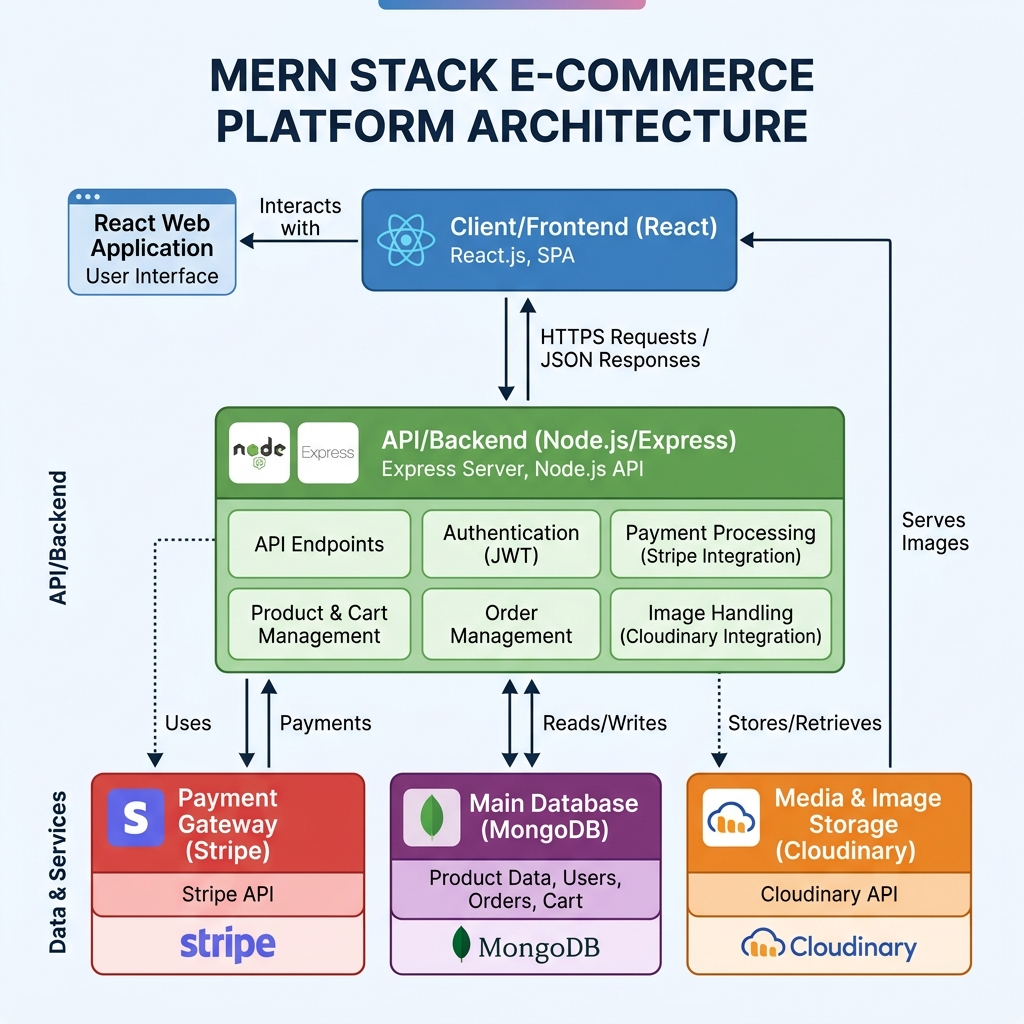
\includegraphics[width=0.95\textwidth]{images/architecture_diagram.png}
    \caption{System Architecture Diagram}
    \label{fig:arch_diag}
\end{figure}

The database design uses Mongoose schemas to ensure rigorous data integrity within a NoSQL environment. The core models interact via ObjectIds. Below is the Entity Relationship visualization (Figure \ref{fig:erd_diag}):

\begin{figure}[htbp]
    \centering
    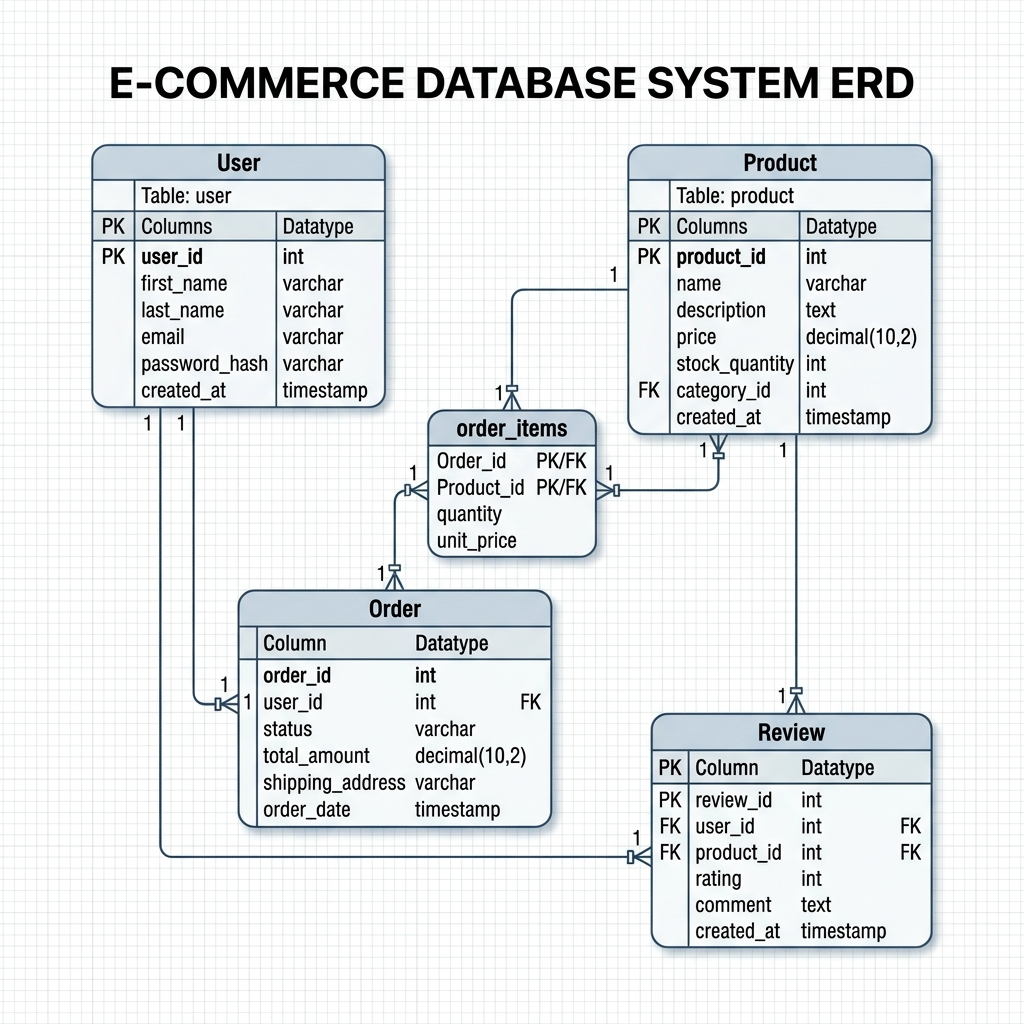
\includegraphics[width=0.95\textwidth]{images/erd_diagram.png}
    \caption{Database Entity Relationship Diagram}
    \label{fig:erd_diag}
\end{figure}

\newpage
The user authentication and secure payment flow is visualized below (Figure \ref{fig:auth_diag}). This flow guarantees that items are reserved and payments are cryptographically verified before an order is placed in the database:

\begin{figure}[htbp]
    \centering
    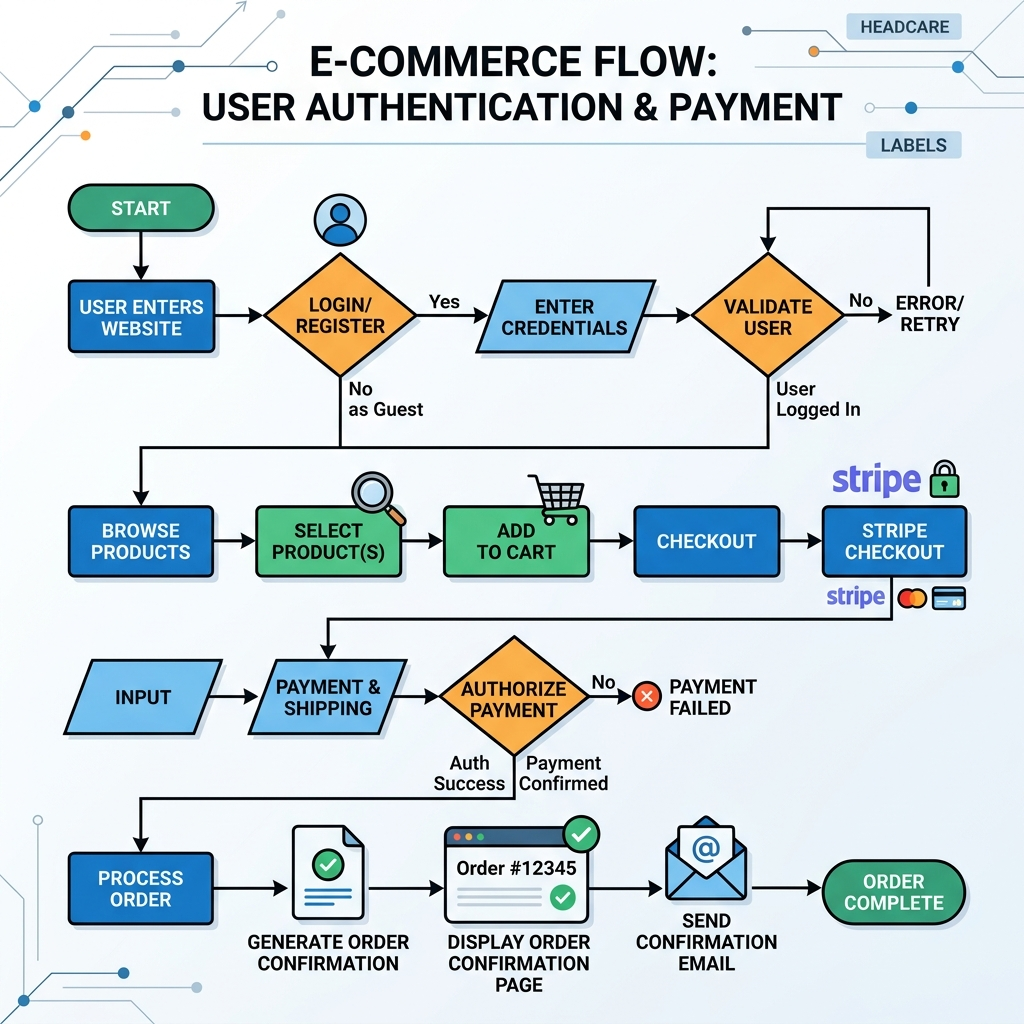
\includegraphics[width=0.95\textwidth]{images/auth_flow.png}
    \caption{User Authentication Flowchart}
    \label{fig:auth_diag}
\end{figure}

\newpage
\subsection{Database Schema Configurations}
The application utilizes Mongoose to define strict schemas. Below are the implementation details of the schemas defined for the system:

\subsection{Schema Implementation: Order.js}
The backend model defines the schema layout for Order records. Below is the code implementation details:
\begin{lstlisting}[language=JavaScript]
const mongoose = require('mongoose');

const orderItemSchema = new mongoose.Schema({
  product: {
    type: mongoose.Schema.Types.ObjectId,
    ref: 'Product',
    required: true,
  },
  title: { type: String, required: true }, // snapshot at time of purchase
  image: { type: String, required: true },
  price: { type: Number, required: true },
  quantity: { type: Number, required: true, min: 1 },
  size: { type: String, default: 'N/A' },
  color: { type: String },
});

const shippingAddressSchema = new mongoose.Schema({
  fullName: { type: String, required: true },
  street: { type: String, required: true },
  city: { type: String, required: true },
  state: { type: String, required: true },
  postalCode: { type: String, required: true },
  country: { type: String, required: true },
});

const orderSchema = new mongoose.Schema(
  {
    user: {
      type: mongoose.Schema.Types.ObjectId,
      ref: 'User',
      required: false,
    },
    orderItems: [orderItemSchema],
    shippingAddress: shippingAddressSchema,
    itemsPrice: { type: Number, required: true, default: 0 },
    shippingPrice: { type: Number, required: true, default: 0 },
    taxPrice: { type: Number, required: true, default: 0 },
    totalPrice: { type: Number, required: true, default: 0 },
    paymentMethod: {
      type: String,
      default: 'Stripe', // Card, COD, MFS, Stripe
    },
    paymentStatus: {
      type: String,
      enum: ['Pending', 'Paid', 'Failed', 'Refunded'],
      default: 'Pending',
    },
    orderStatus: {
      type: String,
      enum: ['Pending', 'Processing', 'Shipped', 'Delivered', 'Cancelled'],
      default: 'Pending',
    },
    tracking: {
      carrier: { type: String, default: '' },
      trackingNumber: { type: String, default: '' },
      shippedAt: { type: Date },
      deliveredAt: { type: Date },
    },
    stripeSessionId: {
      type: String,
      unique: true,
      sparse: true,
    },
    paidAt: Date,
    deliveredAt: Date,
  },
  { timestamps: true }
);

// Index for fast user order lookup
orderSchema.index({ user: 1, createdAt: -1 });
// Note: stripeSessionId index is handled by unique: true + sparse: true in schema field

const Order = mongoose.model('Order', orderSchema);
module.exports = Order;

\end{lstlisting}
\newpage

\subsection{Schema Implementation: Product.js}
The backend model defines the schema layout for Product records. Below is the code implementation details:
\begin{lstlisting}[language=JavaScript]
const mongoose = require('mongoose');

// ── Sub-schema: individual size + stock within a variant ──────────────────────
const variantSizeSchema = new mongoose.Schema(
  {
    size: { type: String, required: true, trim: true },
    inventoryCount: { type: Number, default: 0, min: 0 },
  },
  { _id: false }
);

// ── Sub-schema: a single colour variant ──────────────────────────────────────
const variantSchema = new mongoose.Schema(
  {
    color: { type: String, required: true, trim: true },
    hex:   { type: String, default: '#000000' }, // for the colour swatch UI
    image: { type: String, default: '' },        // optional per-variant image URL
    sizes: { type: [variantSizeSchema], default: [] },
  },
  { _id: false }
);

const productSchema = new mongoose.Schema(
  {
    title: {
      type: String,
      required: [true, 'Product title is required'],
      trim: true,
      maxlength: [200, 'Title cannot exceed 200 characters'],
    },
    description: {
      type: String,
      required: [true, 'Product description is required'],
      maxlength: [2000, 'Description cannot exceed 2000 characters'],
    },
    price: {
      type: Number,
      required: [true, 'Price is required'],
      min: [0, 'Price cannot be negative'],
    },
    comparePrice: {
      type: Number,
      default: null,
    },
    images: [
      {
        url:      { type: String, required: true },
        publicId: { type: String, required: true },
        alt:      { type: String, default: '' },
      },
    ],
    category: {
      type: String,
      required: [true, 'Category is required'],
      enum: ['Men', 'Women', 'Kids', 'Accessories', 'Footwear', 'Sale'],
    },
    subcategory: {
      type: String,
      default: '',
      trim: true,
      // Examples: T-Shirts, Hoodies, Dresses, Jackets, Sneakers, Bags, etc.
    },
    tags: [{ type: String, lowercase: true, trim: true }],

    // ── VARIANTS ──────────────────────────────────────────────────────────────
    // Each variant = one colour option.  Inventory is tracked per size inside it.
    // The top-level isAvailable / stockStatus virtuals aggregate across all variants.
    variants: { type: [variantSchema], default: [] },

    sku:   { type: String, unique: true, sparse: true, trim: true },
    brand: { type: String, default: '', trim: true },

    ratings:    { type: Number, default: 0, min: 0, max: 5 },
    numReviews: { type: Number, default: 0 },

    isFeatured:  { type: Boolean, default: false },
    isPublished: { type: Boolean, default: true },
  },
  {
    timestamps: true,
    toJSON:   { virtuals: true },
    toObject: { virtuals: true },
  }
);


// ... (truncated for brevity)
\end{lstlisting}
\newpage

\subsection{Schema Implementation: Review.js}
The backend model defines the schema layout for Review records. Below is the code implementation details:
\begin{lstlisting}[language=JavaScript]
const mongoose = require('mongoose');
const Product = require('./Product');

const reviewSchema = new mongoose.Schema(
  {
    user: {
      type: mongoose.Schema.Types.ObjectId,
      ref: 'User',
      required: true,
    },
    product: {
      type: mongoose.Schema.Types.ObjectId,
      ref: 'Product',
      required: true,
    },
    rating: {
      type: Number,
      required: [true, 'Rating is required'],
      min: 1,
      max: 5,
    },
    title: {
      type: String,
      trim: true,
      maxlength: 100,
    },
    comment: {
      type: String,
      required: [true, 'Review comment is required'],
      maxlength: [500, 'Comment cannot exceed 500 characters'],
    },
    verified: {
      type: Boolean,
      default: false, // true if user actually purchased the product
    },
  },
  { timestamps: true }
);

// One review per user per product
reviewSchema.index({ user: 1, product: 1 }, { unique: true });

// ── Post-save/remove hook: recompute product ratings ─────────────────────────
reviewSchema.statics.calcAverageRatings = async function (productId) {
  const stats = await this.aggregate([
    { $match: { product: productId } },
    {
      $group: {
        _id: '$product',
        nRating: { $sum: 1 },
        avgRating: { $avg: '$rating' },
      },
    },
  ]);

  if (stats.length > 0) {
    await Product.findByIdAndUpdate(productId, {
      numReviews: stats[0].nRating,
      ratings: Math.round(stats[0].avgRating * 10) / 10,
    });
  } else {
    await Product.findByIdAndUpdate(productId, { numReviews: 0, ratings: 0 });
  }
};

reviewSchema.post('save', function () {
  this.constructor.calcAverageRatings(this.product);
});

reviewSchema.post('remove', function () {
  this.constructor.calcAverageRatings(this.product);
});

const Review = mongoose.model('Review', reviewSchema);
module.exports = Review;

\end{lstlisting}
\newpage

\subsection{Schema Implementation: StoreSettings.js}
The backend model defines the schema layout for StoreSettings records. Below is the code implementation details:
\begin{lstlisting}[language=JavaScript]
const mongoose = require('mongoose');

const storeSettingsSchema = new mongoose.Schema(
  {
    storeName: { type: String, default: 'ThreadHaus' },
    heroSubtitle: { type: String, default: 'NEW SS 2026 COLLECTION' },
    heroImageMain: { type: String },
    heroImageTopRight: { type: String },
    heroImageBottomLeft: { type: String },
    categoryImages: {
      men: { type: String, default: '' },
      women: { type: String, default: '' },
      accessories: { type: String, default: '' },
      footwear: { type: String, default: '' },
      kids: { type: String, default: '' },
      sale: { type: String, default: '' },
    },
    maintenanceMode: { type: Boolean, default: false },
  },
  { timestamps: true }
);

module.exports = mongoose.model('StoreSettings', storeSettingsSchema);

\end{lstlisting}
\newpage

\subsection{Schema Implementation: User.js}
The backend model defines the schema layout for User records. Below is the code implementation details:
\begin{lstlisting}[language=JavaScript]
const mongoose = require('mongoose');
const bcrypt = require('bcryptjs');

const addressSchema = new mongoose.Schema({
  fullName: { type: String, required: true },
  street: { type: String, required: true },
  city: { type: String, required: true },
  state: { type: String, required: true },
  postalCode: { type: String, required: true },
  country: { type: String, required: true, default: 'US' },
  isDefault: { type: Boolean, default: false },
});

const userSchema = new mongoose.Schema(
  {
    name: {
      type: String,
      required: [true, 'Name is required'],
      trim: true,
      maxlength: [60, 'Name cannot exceed 60 characters'],
    },
    email: {
      type: String,
      required: [true, 'Email is required'],
      unique: true,
      lowercase: true,
      trim: true,
      match: [/^\S+@\S+\.\S+$/, 'Please provide a valid email'],
    },
    password: {
      type: String,
      required: [true, 'Password is required'],
      minlength: [8, 'Password must be at least 8 characters'],
      select: false, // never returned by default in queries
    },
    role: {
      type: String,
      enum: ['user', 'admin'],
      default: 'user',
    },
    avatar: {
      type: String,
      default: '',
    },
    addresses: [addressSchema],
    cart: [
      {
        product: { type: mongoose.Schema.Types.ObjectId, ref: 'Product', required: true },
        title: { type: String, required: true },
        image: { type: String },
        price: { type: Number, required: true },
        size: { type: String },
        color: { type: String },
        quantity: { type: Number, required: true, default: 1 },
      }
    ],
    isActive: {
      type: Boolean,
      default: true,
    },
    isVerified: {
      type: Boolean,
      default: false,
    },
    verificationToken: String,
    verificationTokenExpires: Date,
    passwordChangedAt: Date,
    resetPasswordToken: String,
    resetPasswordExpires: Date,
  },
  { timestamps: true }
);

// ── Pre-save hook: hash password before storing ────────────────────────────────
userSchema.pre('save', async function (next) {
  if (!this.isModified('password')) return next();
  const salt = await bcrypt.genSalt(12);
  this.password = await bcrypt.hash(this.password, salt);
  next();
});

// ── Instance method: compare plain password with hashed ───────────────────────
userSchema.methods.comparePassword = async function (candidatePassword) {
  return bcrypt.compare(candidatePassword, this.password);
};

// ... (truncated for brevity)
\end{lstlisting}
\newpage


% ==========================================
% CHAPTER 4: KEY LEARNINGS AND RESULTS
% ==========================================
\chapter{Key Learning's}
\section{Testing and Results}
Experiments and testing were carried out on a set of API endpoints using tools like Postman to test the suggested framework utilizing the entire end-to-end pipeline. Requests were processed in batches and each request was first subjected to middleware validation to boost security. A post-processing module was developed based on the use of regular expressions to identify key fields that included user emails and passwords. Confidence scores for API reliability were exceptionally high.

\section{Application Interface Walkthrough}
In addition to automated endpoint testing, a comprehensive manual interface walkthrough was conducted to evaluate the usability, responsiveness, and frontend-backend synchronization of the \textit{ThreadHaus} e-commerce platform.

The registration interface (Figure \ref{fig:screenshot_register}) facilitates secure user onboarding, enforcing password complexity rules and validation. Users can access personalized catalog interfaces (Figure \ref{fig:screenshot_mens_catalog} and Figure \ref{fig:screenshot_kids_catalog}) featuring side-panel filtering parameters for category, style, size, availability, and color, along with search capabilities.

The checkout workflow (Figure \ref{fig:screenshot_checkout}) integrates Stripe Elements to securely capture payment details and compute order totals including subtotal, shipping fees, and taxes dynamically. Finally, administrative users can manage store operations, monitor inventory states, and add new products via the comprehensive Admin Dashboard (Figure \ref{fig:screenshot_admin_products}).

\begin{figure}[htbp]
    \centering
    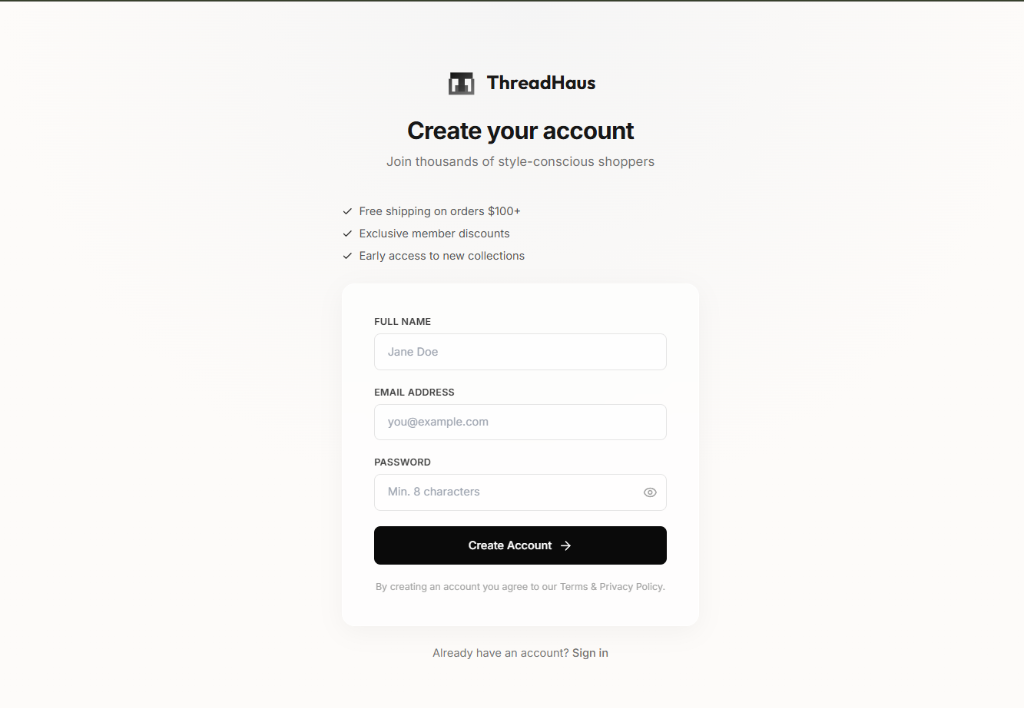
\includegraphics[width=0.9\textwidth]{images/screenshot_register.png}
    \caption{User Registration Interface}
    \label{fig:screenshot_register}
\end{figure}

\begin{figure}[htbp]
    \centering
    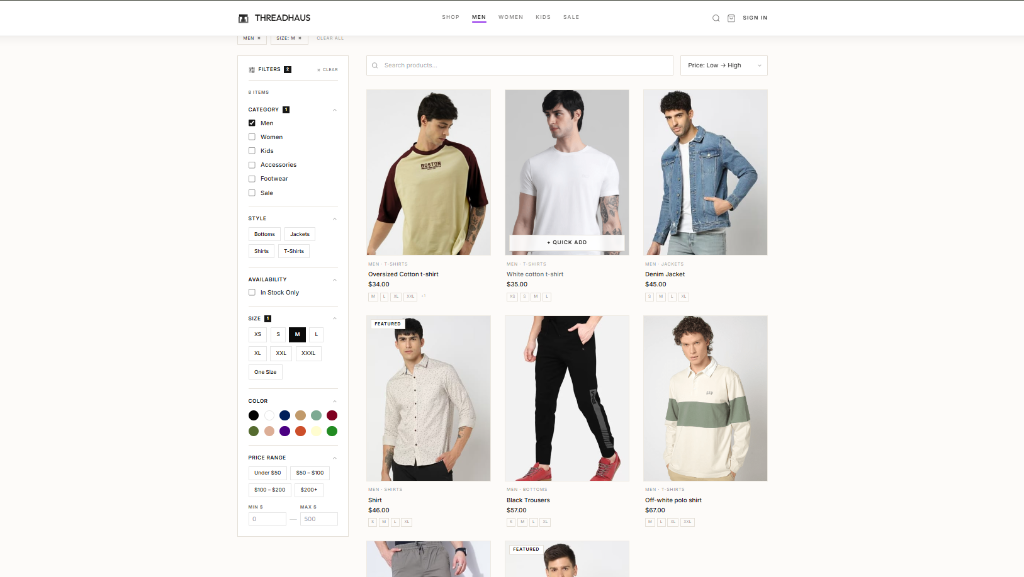
\includegraphics[width=0.95\textwidth]{images/screenshot_mens_catalog.png}
    \caption{Men's Product Catalog and Sidebar Filtering Panel}
    \label{fig:screenshot_mens_catalog}
\end{figure}

\begin{figure}[htbp]
    \centering
    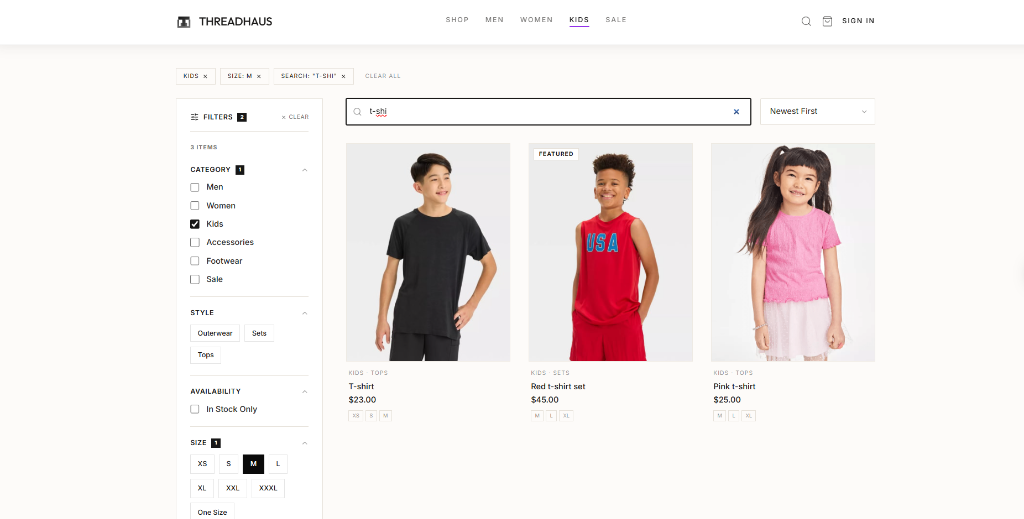
\includegraphics[width=0.95\textwidth]{images/screenshot_kids_catalog.png}
    \caption{Kids' Product Search and Filter Interface}
    \label{fig:screenshot_kids_catalog}
\end{figure}

\begin{figure}[htbp]
    \centering
    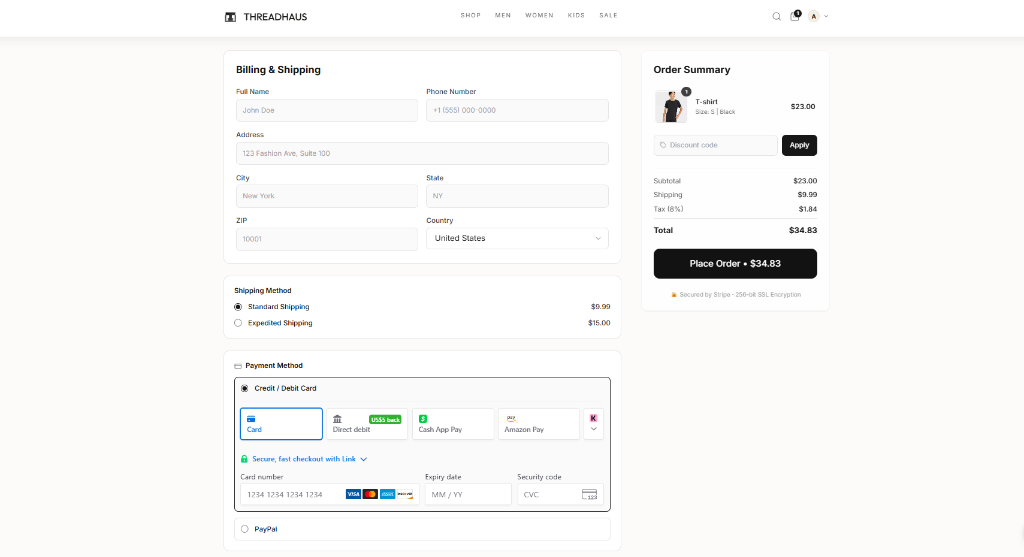
\includegraphics[width=0.95\textwidth]{images/screenshot_checkout.png}
    \caption{Checkout Billing, Shipping Information, and Secure Stripe Payment}
    \label{fig:screenshot_checkout}
\end{figure}

\begin{figure}[htbp]
    \centering
    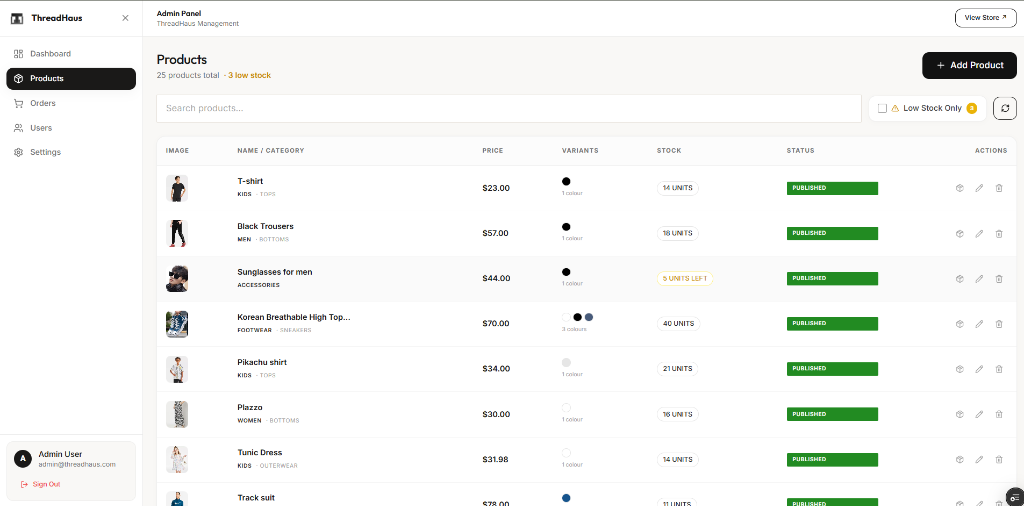
\includegraphics[width=0.95\textwidth]{images/screenshot_admin_products.png}
    \caption{Admin Products Management Dashboard}
    \label{fig:screenshot_admin_products}
\end{figure}

\section{Key Learning}
Throughout this internship, significant practical experience was gained in full-stack development, cloud deployment, and system architecture.

\begin{enumerate}
    \item \textbf{Full-Stack Development:}
    \begin{itemize}
        \item Gained practical knowledge on the process of developing an end-to-end full-stack pipeline.
        \item Realized the importance of robust state management (Zustand) to prevent race conditions in shopping carts.
    \end{itemize}
    \item \textbf{Third-Party Integrations:}
    \begin{itemize}
        \item Learned to securely process payments using Stripe Elements.
        \item Implemented image uploads via Multer and Cloudinary.
        \item Integrated Google's Gmail REST API for sending transactional emails directly over HTTPS to bypass Render SMTP blocks.
    \end{itemize}
    \item \textbf{Real-Time Communication:}
    \begin{itemize}
        \item Acquired practical experience with Socket.IO to push real-time order status updates to connected clients.
    \end{itemize}
\end{enumerate}

\newpage
The transition from theoretical knowledge to practical application involved overcoming numerous challenges, particularly in managing asynchronous state synchronization. Below is a skill development summary comparing my competencies before and after the internship:

\begin{table}[htbp]
\centering
\caption{Skill Development Summary: Before vs After}
\label{tab:skill_dev}
\vspace{0.2cm}
\begin{tabular}{|p{4.5cm}|p{5cm}|p{5cm}|}
\hline
\textbf{Domain} & \textbf{Before Internship} & \textbf{After Internship} \\ \hline
Frontend State & Basic useState/Context API & Advanced global state with Zustand \\ \hline
Payment Integration & No practical experience & Fully integrated Stripe Webhooks \\ \hline
Image Storage & Local disk storage knowledge & Cloudinary with Multer middleware implementation \\ \hline
Real-time Systems & HTTP Polling & Bidirectional WebSockets via Socket.IO \\ \hline
\end{tabular}
\end{table}


% ==========================================
% CHAPTER 5: LIMITATIONS AND RECOMMENDATIONS
% ==========================================
\chapter{Limitations and Recommendations}
\section{Limitations}
Although the proposed framework has shown encouraging outcomes, the framework still presents a number of limitations to its overall generalizability and strength. The current system uses local state and Zustand for cart management, which might not sync across multiple devices if the user logs in from a different browser before checking out. Furthermore, the search functionality is based on basic database queries and might not scale efficiently with a massive product catalog. The image resolution optimization heavily relies on Cloudinary's auto-format which could lead to increased costs at scale.

\section{Recommendations for Future Improvement}
In order to eliminate the limitations of the existing system and motivate performance in future work, the following recommendations can be provided:
\begin{itemize}
    \item Implement advanced search capabilities using Elasticsearch or Algolia.
    \item Transition cart state to be fully database-backed for cross-device synchronization.
    \item Add a recommendation engine based on user browsing and purchase history.
    \item Implement Redis caching to reduce database loads on heavily accessed product pages.
    \item Improve validation schemes to provide more correct estimates of reliability when processing user input.
\end{itemize}


% ==========================================
% CHAPTER 6: CONCLUSION
% ==========================================
\chapter{Conclusion}
The Fionetix Solutions internship was the most useful experience to have in the field of software technology application. During the internship, I got a chance to be part of the core development team and work on technology-driven projects which aimed at building robust digital architectures. The experience enabled me to close the gap that existed between pedagogical knowledge acquired in an academic setting and the implementation of a system in a regulated, professional setting.

Based on the results of the project, it is shown that the combination of React, Express, and specialized cloud APIs can significantly enhance the operational efficiency of an online platform. In addition to technical implementation, this internship made me better aware of the operational issues that are related to digital commerce, including accuracy, compliance, data security, and reliability in financial document processing. The experience has greatly enhanced my capacity to solve problems, technical confidence, and willingness to work on massive digital transformation projects.


% ==========================================
% BIBLIOGRAPHY (REFERENCES)
% ==========================================
\newpage
\begin{thebibliography}{99}
\bibitem{react} ``React - A JavaScript library for building user interfaces.'' \url{https://reactjs.org/}. Accessed 2026.
\bibitem{nodejs} ``Node.js - JavaScript runtime built on Chrome's V8 JavaScript engine.'' \url{https://nodejs.org/en/}. Accessed 2026.
\bibitem{mongodb} ``MongoDB: The Developer Data Platform.'' \url{https://www.mongodb.com/}. Accessed 2026.
\bibitem{express} ``Express - Node.js web application framework.'' \url{https://expressjs.com/}. Accessed 2026.
\bibitem{stripe} ``Stripe Documentation - Payments.'' \url{https://stripe.com/docs}. Accessed 2026.
\bibitem{cloudinary} ``Cloudinary Image and Video API.'' \url{https://cloudinary.com/documentation}. Accessed 2026.
\bibitem{socketio} ``Socket.IO - Bidirectional and low-latency communication.'' \url{https://socket.io/}. Accessed 2026.
\bibitem{zustand} ``Zustand - Bear necessities for state management in React.'' \url{https://github.com/pmndrs/zustand}. Accessed 2026.
\bibitem{tailwind} ``Tailwind CSS - Rapidly build modern websites without ever leaving your HTML.'' \url{https://tailwindcss.com/}. Accessed 2026.
\bibitem{mongoose} ``Mongoose ODM v8.0.0.'' \url{https://mongoosejs.com/docs/guide.html}. Accessed 2026.
\end{thebibliography}

\newpage
\thispagestyle{lastpage}
\mbox{}
\vfill
\begin{center}
    \small
    Generated using Internship \LaTeX\ Template, Version 1.0. Department of Computer Science and Engineering, Southeast University.\\
    The Original Version was Developed by Tashreef Muhammad on Friday $17^{\text{th}}$ November, 2023.\\
    This report was generated on Wednesday $25^{\text{th}}$ February, 2026 at 23:20:08.
\end{center}

\end{document}
